\section{Overview of Bolt}

\textbf{Bolt} is a congestion-control algorithm designed for ultra-low-latency data center networks. The central idea of Bolt is that conventional RTT-scale control reacts too slowly when line rates are high and many transfers are only a few BDPs long. In such settings, even a small delay in congestion response can create unnecessary queueing, while slow ramp-up after bandwidth becomes available can cause under-utilization.

\subsection{Impact of the Problem in Data Centers}

At high link speeds, congestion builds faster than RTT-scale control can respond. A sender may continue injecting packets even after the bottleneck has already started queueing, which creates avoidable delay. This effect becomes more severe when many flows are short, because a large fraction of traffic finishes before conventional feedback fully converges.

Another problem appears when a flow finishes and frees bandwidth. The remaining flows do not immediately increase their sending rate, since the increase is still governed by delayed ACK-driven control. As a result, the link stays temporarily under-utilized even though capacity is available.

The paper shows that these two effects become fundamental at modern data center rates: queue can form within a fraction of an RTT, and freed bandwidth can remain unused for multiple RTTs. Bolt is designed to reduce both excess queueing and post-completion under-utilization.

\begin{figure}[t]
\centering
\includegraphics[width=0.9\linewidth]{fig3}
\caption{Use Bolt paper Figure 3 here.}
\label{fig:bolt-fig3}
\end{figure}

\begin{figure}[t]
\centering
\includegraphics[width=0.9\linewidth]{fig4}
\caption{Use Bolt paper Figure 4 here.}
\label{fig:bolt-fig4}
\end{figure}

\begin{figure}[t]
\centering
\includegraphics[width=0.9\linewidth]{fig5}
\caption{Use Bolt paper Figure 5 here.}
\label{fig:bolt-fig5}
\end{figure}

\subsection{Mechanisms Used to Mitigate the Problem}

Bolt mitigates these problems using three mechanisms: \textbf{Sub-RTT Control (SRC)}, \textbf{Proactive Ramp-Up (PRU)}, and \textbf{Supply Matching (SM)}.

\paragraph{Sub-RTT Control (SRC)}
SRC reduces control-loop delay by generating congestion feedback at the bottleneck instead of waiting for receiver-driven reflection. When queue occupancy reaches the congestion threshold, the switch generates a feedback packet and sends it directly to the sender. The sender then decreases its congestion window using the SRC feedback delay and the measured queue.

\textbf{Switch and sender logic:}
\begin{enumerate}
\item For each arriving data packet, compute the current queue occupancy at the switch.
\item If the queue occupancy is at least the congestion threshold and the packet is not already marked for decrease, create an SRC packet carrying queue size, link rate, and the packet transmission timestamp.
\item Set the packet decrease mark and clear its increase mark so that downstream switches do not generate another SRC for the same packet.
\item At the sender, compute the SRC feedback delay from the original data transmission time and the SRC arrival time.
\item Use the ratio between flow rate and congested-link rate to determine the target queue contribution of the flow.
\item If enough time has passed since the last decrease, reduce the congestion window by one packet.
\end{enumerate}

\paragraph{Proactive Ramp-Up (PRU)}
PRU reduces the slow recovery that follows flow completion. When a flow is about to finish, packets in its last window are marked so that switches can account for the bandwidth that will be released in the next RTT. That bandwidth is represented as PRU tokens and assigned to continuing flows.

\textbf{Switch and sender logic:}
\begin{enumerate}
\item When the remaining unsent data of a flow becomes at most one current congestion window, mark outgoing packets with the LAST flag.
\item If such a packet is not from the first congestion window of the flow, the switch increases the PRU token count for the egress port.
\item Continuing flows mark outgoing packets with the INC flag to request permission for window growth.
\item If a switch has PRU tokens available, it keeps the INC flag and consumes one PRU token.
\item If no switch on the path clears the INC flag, the receiver reflects the flag in the ACK.
\item On receiving such an ACK, the sender increases the congestion window by one packet.
\end{enumerate}

\paragraph{Supply Matching (SM)}
SM keeps sender demand aligned with actual bottleneck supply. The switch tracks the difference between how many bytes the link could have transmitted and how many bytes actually arrived. This difference is stored as a supply token and is used to allow or deny increase requests.

\textbf{Switch logic:}
\begin{enumerate}
\item On each data-packet arrival, compute inter-arrival time using the current time and the previous packet-arrival time for that egress port.
\item Compute available supply as link bandwidth multiplied by inter-arrival time.
\item Compute demand as the size of the arriving packet.
\item Update the supply token as the previous token plus supply minus demand.
\item Cap the supply token at one MTU.
\item When a packet requests increase and no PRU token is available, keep the INC flag only if the supply token is at least one MTU.
\item If increase is granted through supply matching, decrease the supply token by one MTU.
\item Otherwise, clear the INC flag so the sender does not grow its window.
\end{enumerate}

Together, SRC reduces delayed congestion reaction, PRU reduces post-completion under-utilization, and SM keeps window growth aligned with available bandwidth. These three mechanisms form the core algorithmic contribution of Bolt.

\section{Core Implementation in ns-3}

The reusable implementation of Bolt in ns-3 is concentrated in the \texttt{src/internet/model} directory, with module registration completed in \texttt{src/internet/CMakeLists.txt}. This part contains the protocol definition, sender-side control logic, switch-side control logic, and the integration path needed to carry switch feedback back to the sender. The scratch files used for simulation are not part of this core implementation and are therefore excluded from this section.

\subsection{\texttt{src/internet/CMakeLists.txt}}

This file registers the Bolt implementation as part of the ns-3 Internet module. The source and header entries for \texttt{bolt-header}, \texttt{bolt-queue}, and \texttt{tcp-bolt} are added here so that the new protocol components are compiled together with the existing Internet stack. Without this registration step, the Bolt implementation would remain unavailable to the simulator even if the model files were present.

\subsection{\texttt{src/internet/model/bolt-header.h} and \texttt{bolt-header.cc}}

These files define the Bolt control header and its packet format. The header carries the control fields required by the algorithm, including source and destination ports, sequence information, queue drain time, reflected delay, and the Bolt control flags. The flags include the markers required by the paper, such as \texttt{BTS}, \texttt{LAST}, \texttt{FIRST}, \texttt{INCWIN}, and \texttt{DECWIN}. Serialization and deserialization logic are implemented in the same component so that Bolt control information can be inserted into packets, transmitted through the network, and recovered correctly at the receiving side. This file therefore provides the common data format shared by the sender, switch, and feedback path.

\subsection{\texttt{src/internet/model/tcp-bolt.h} and \texttt{tcp-bolt.cc}}

These files implement the sender-side Bolt algorithm as a new TCP congestion-control variant. The class \texttt{TcpBolt} is defined as a subclass of \texttt{TcpCongestionOps}, which allows Bolt to operate within the standard ns-3 TCP framework while replacing the normal congestion-control behavior with the logic described in the paper.

The main sender-side mechanisms are implemented here. The method \texttt{ProcessSrcPacket()} handles SRC feedback generated by the bottleneck and performs the corresponding congestion-window reduction. The method \texttt{ProcessIncFlag()} handles reflected increase permission carried by acknowledgments and performs controlled window growth. The method \texttt{ShouldRequestInc()} determines when an outgoing data segment should request an increase opportunity by setting the corresponding Bolt control flag. The conventional additive-increase behavior is intentionally not used inside \texttt{IncreaseWindow()}, because positive growth in Bolt is meant to be governed by explicit feedback rather than by the standard ACK-driven TCP loop. As a result, this file forms the complete end-host realization of the sender logic presented in the Bolt paper.

\subsection{\texttt{src/internet/model/bolt-queue.h} and \texttt{bolt-queue.cc}}

These files implement the switch-side logic of Bolt through a custom queue class named \texttt{BoltQueue}. This component is responsible for observing packets at the bottleneck and applying the three core mechanisms of the algorithm: SRC, PRU, and SM.

When a data packet arrives, the queue extracts the embedded \texttt{BoltHeader} from the packet payload and examines the control flags. If the queue occupancy crosses the configured congestion threshold, \texttt{GenerateSrcPacket()} creates a switch-to-sender feedback packet and marks the original packet with the decrease flag. This realizes Sub-RTT Control. For Proactive Ramp-Up, the method \texttt{UpdatePruToken()} updates the PRU token state based on the \texttt{LAST} and \texttt{FIRST} markers carried by packets that belong to a flow's final congestion window. For Supply Matching, the method \texttt{CalculateSupplyToken()} computes the mismatch between available link supply and arriving demand, while \texttt{ProcessIncFlag()} decides whether an increase request should be preserved or cleared according to PRU tokens and SM tokens. The queue also rewrites the Bolt header on in-flight packets whenever the \texttt{INCWIN} or \texttt{DECWIN} state must be changed. Therefore, this file contains the main bottleneck-side realization of the Bolt control logic.

\subsection{\texttt{src/internet/model/tcp-socket-base.h} and \texttt{tcp-socket-base.cc}}

These files provide the integration path that delivers external Bolt feedback into the sender-side congestion-control module. The core addition is the method \texttt{ProcessExternalSrcPacket()}, which accepts an SRC packet, decodes its Bolt control information, and passes the relevant fields to \texttt{TcpBolt::ProcessSrcPacket()}. An overloaded version also accepts an explicit link rate so that external adapters can preserve the sender-side control law even when the underlying medium does not use the same built-in rate encoding as the wired Bolt path.

This component also exposes \texttt{GetCongestionControlAlgorithm()}, which makes the active TCP congestion-control object accessible when integration with Bolt-specific feedback handling is required. The purpose of this file is not to redefine the Bolt algorithm itself, but to provide the transport-layer plumbing needed to connect generated SRC feedback to the sender's congestion controller inside ns-3.

\subsection{\texttt{src/internet/model/ipv4-l3-protocol.cc}}

This file contains the IP-layer support needed to recognize and return Bolt SRC packets. When an incoming packet is identified as carrying a Bolt header with the \texttt{BTS} flag set, the IP-layer logic treats it as switch-generated feedback rather than as ordinary payload. The implementation then swaps the source and destination IP addresses and forwards the packet back toward the original sender. This allows SRC feedback generated at the bottleneck to travel through the simulator as an explicit control packet and reach the sender through the normal protocol stack.

In this way, the IP layer provides a forwarding path for Bolt feedback, while the queue and transport components implement the control decisions themselves.

\section{Wired Results}

The wired experiment evaluates Bolt over a fixed bottleneck link while varying the number of nodes, the number of flows, and the packet generation rate. The measured metrics are throughput, average end-to-end delay, packet delivery ratio, and packet drop ratio.

\subsection{Node Sweep}

\begin{table}[t]
\centering
\small
\caption{Wired results for node variation.}
\label{tab:wired-nodes}
\begin{tabular}{ccccc}
\hline
Nodes & Throughput (Mbps) & Delay (ms) & PDR & Drop Ratio \\
\hline
20  & 5.991 & 7.167  & 0.995 & 0.005 \\
40  & 5.991 & 7.167  & 0.995 & 0.005 \\
60  & 5.991 & 7.167  & 0.995 & 0.005 \\
80  & 5.991 & 7.167  & 0.995 & 0.005 \\
100 & 5.991 & 7.167  & 0.995 & 0.005 \\
\hline
\end{tabular}
\end{table}

\begin{figure}[t]
\centering
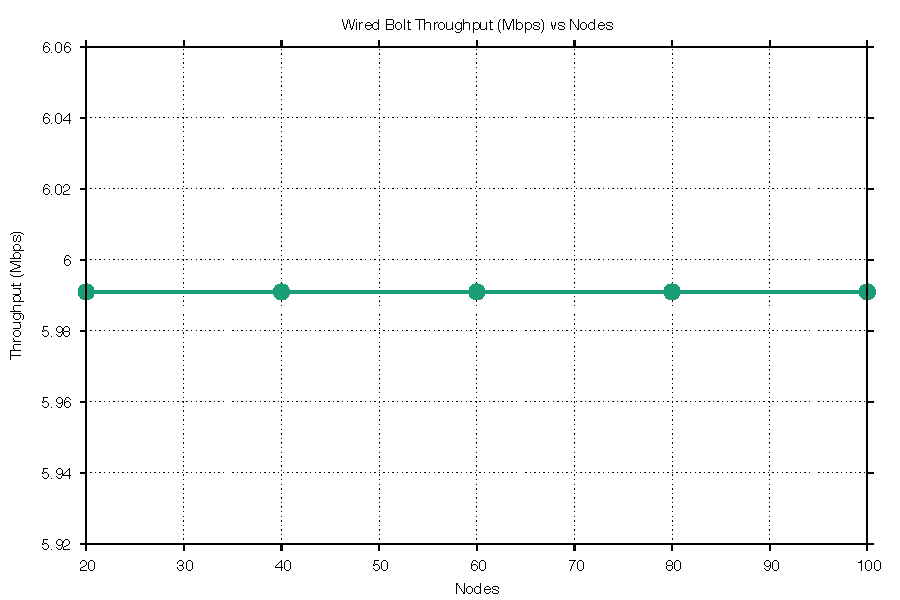
\includegraphics[width=0.78\linewidth]{project7-row7-plots/wired-throughput_mbps-nodes}
\caption{Wired throughput versus number of nodes.}
\label{fig:wired-throughput-nodes}
\end{figure}

\noindent\textbf{Reason:} Throughput stays flat because node count changes the number of hosts, not the single active bottleneck that carries the measured flows.

\begin{figure}[t]
\centering
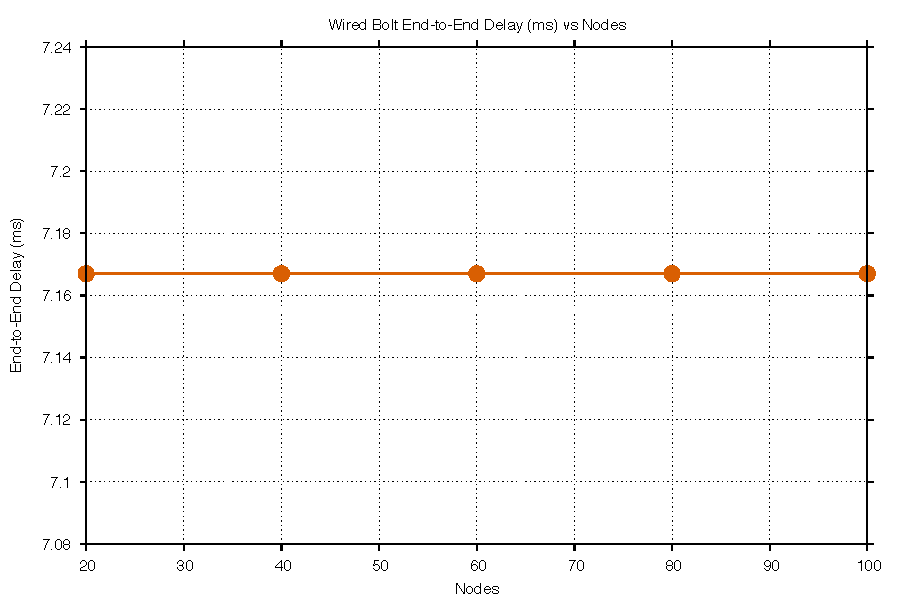
\includegraphics[width=0.78\linewidth]{project7-row7-plots/wired-avg_delay_ms-nodes}
\caption{Wired average delay versus number of nodes.}
\label{fig:wired-delay-nodes}
\end{figure}

\noindent\textbf{Reason:} Delay remains flat because queueing conditions on the fixed bottleneck do not change with extra idle nodes.

\begin{figure}[t]
\centering
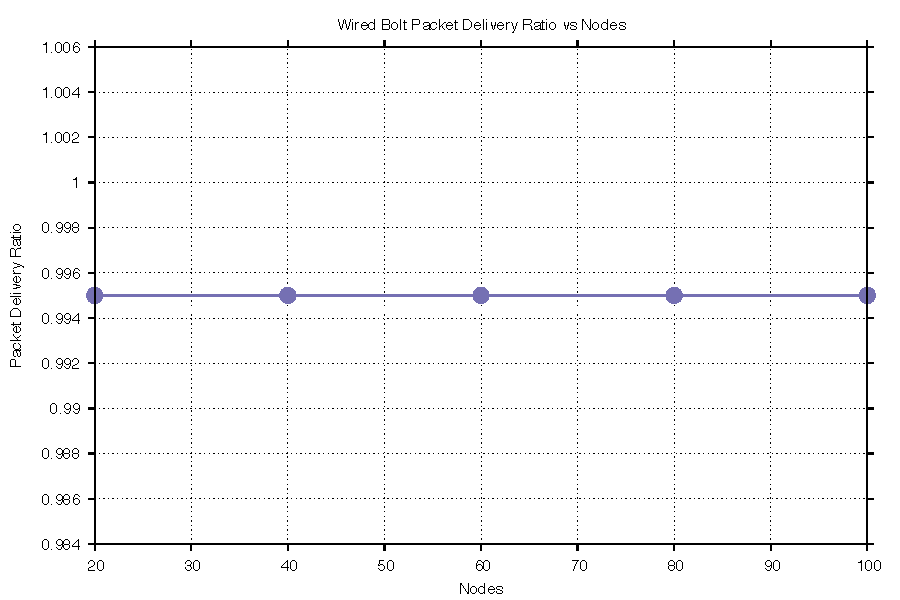
\includegraphics[width=0.78\linewidth]{project7-row7-plots/wired-pdr-nodes}
\caption{Wired packet delivery ratio versus number of nodes.}
\label{fig:wired-pdr-nodes}
\end{figure}

\noindent\textbf{Reason:} PDR stays almost constant because the same bottleneck and the same active load pattern are preserved across node counts.

\begin{figure}[t]
\centering
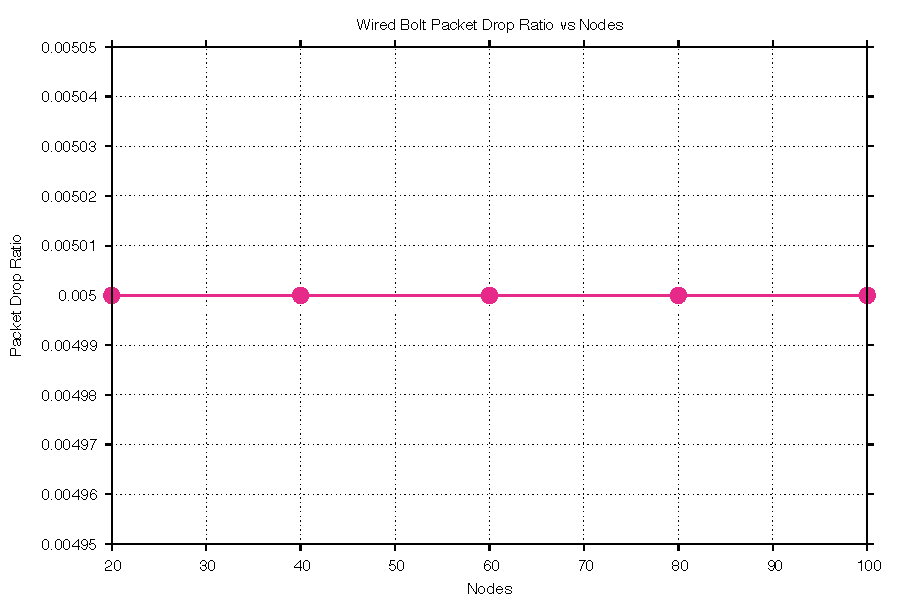
\includegraphics[width=0.78\linewidth]{project7-row7-plots/wired-drop_ratio-nodes}
\caption{Wired packet drop ratio versus number of nodes.}
\label{fig:wired-drop-nodes}
\end{figure}

\noindent\textbf{Reason:} Drop ratio remains nearly unchanged because additional nodes do not create extra congestion on the measured path.

\subsection{Flow Sweep}

\begin{table}[t]
\centering
\small
\caption{Wired results for flow variation.}
\label{tab:wired-flows}
\begin{tabular}{ccccc}
\hline
Flows & Throughput (Mbps) & Delay (ms) & PDR & Drop Ratio \\
\hline
10 & 4.882 & 3.632  & 0.999 & 0.001 \\
20 & 5.991 & 7.167  & 0.995 & 0.005 \\
30 & 8.226 & 17.589 & 0.997 & 0.003 \\
40 & 8.377 & 14.985 & 1.000 & 0.000 \\
50 & 8.905 & 31.661 & 0.995 & 0.005 \\
\hline
\end{tabular}
\end{table}

\begin{figure}[t]
\centering
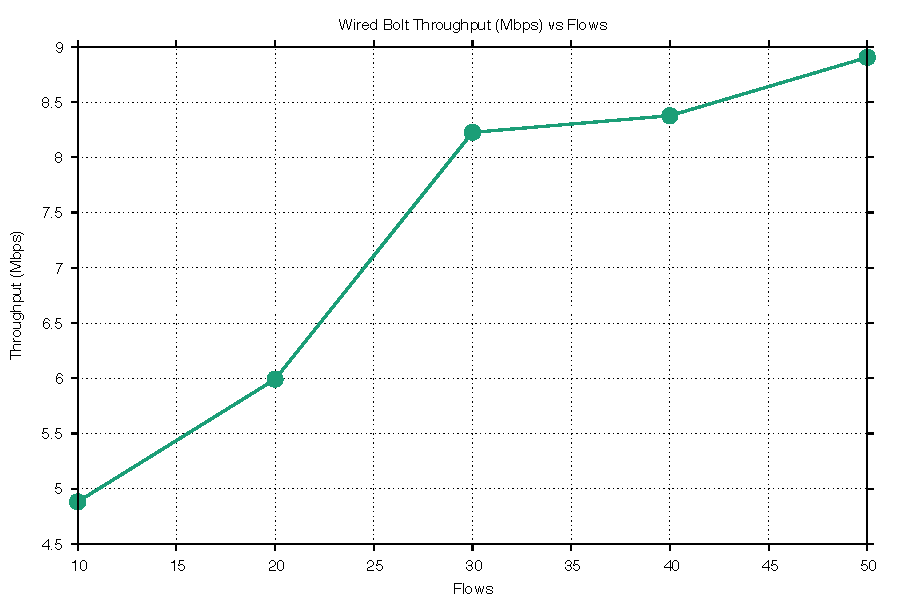
\includegraphics[width=0.78\linewidth]{project7-row7-plots/wired-throughput_mbps-flows}
\caption{Wired throughput versus number of flows.}
\label{fig:wired-throughput-flows}
\end{figure}

\noindent\textbf{Reason:} Throughput increases with flow count because more concurrent flows utilize the bottleneck more effectively until saturation is approached.

\begin{figure}[t]
\centering
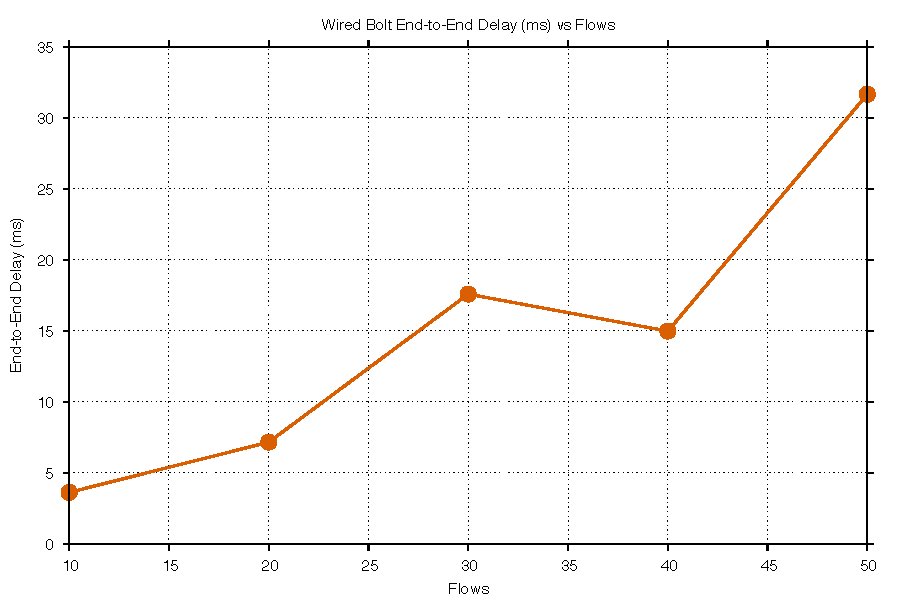
\includegraphics[width=0.78\linewidth]{project7-row7-plots/wired-avg_delay_ms-flows}
\caption{Wired average delay versus number of flows.}
\label{fig:wired-delay-flows}
\end{figure}

\noindent\textbf{Reason:} Delay rises with more flows because heavier contention builds a deeper queue at the bottleneck.

\begin{figure}[t]
\centering
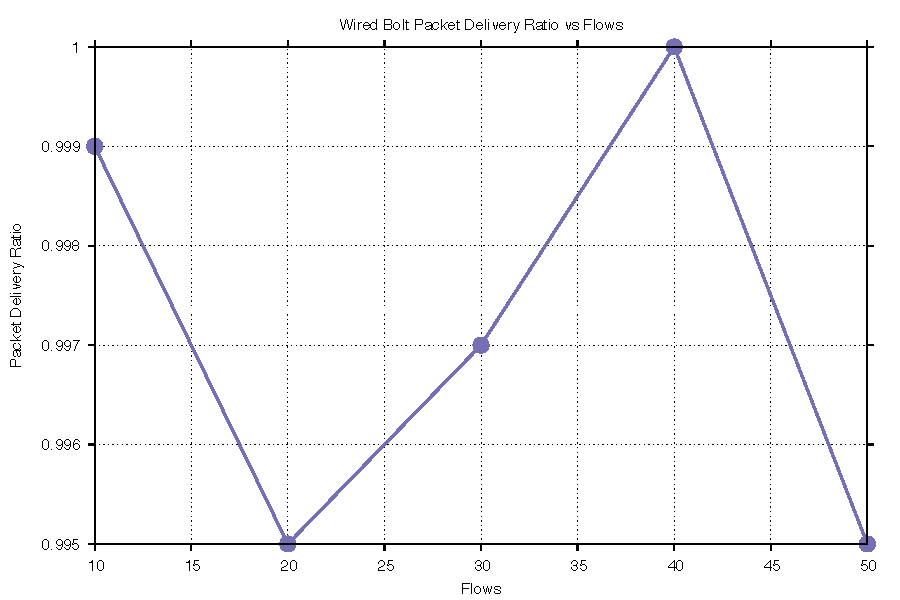
\includegraphics[width=0.78\linewidth]{project7-row7-plots/wired-pdr-flows}
\caption{Wired packet delivery ratio versus number of flows.}
\label{fig:wired-pdr-flows}
\end{figure}

\noindent\textbf{Reason:} PDR remains high because the wired TCP path still delivers almost all packets even under increased load.

\begin{figure}[t]
\centering
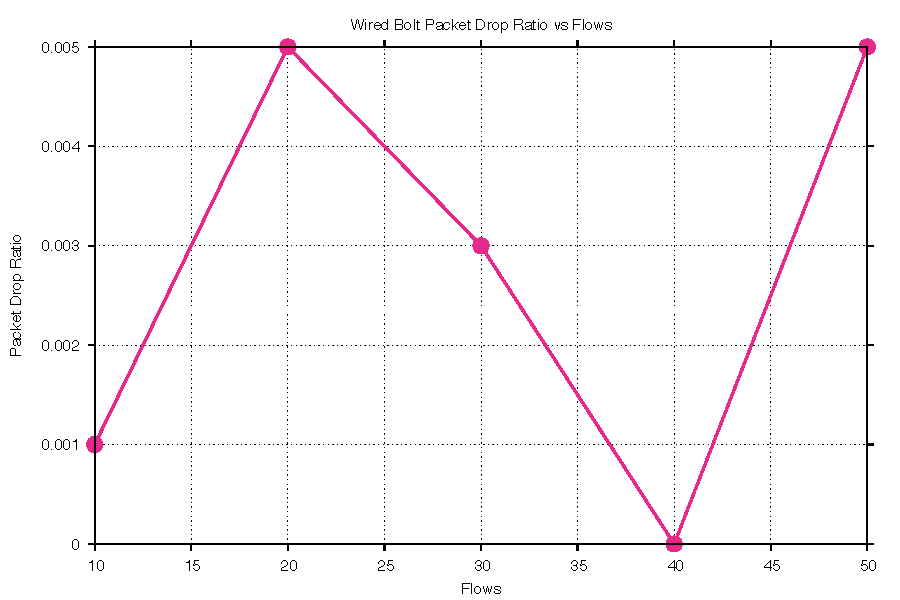
\includegraphics[width=0.78\linewidth]{project7-row7-plots/wired-drop_ratio-flows}
\caption{Wired packet drop ratio versus number of flows.}
\label{fig:wired-drop-flows}
\end{figure}

\noindent\textbf{Reason:} Drop ratio stays very low because losses are limited even when flow count increases.

\subsection{Packet-Rate Sweep}

\begin{table}[t]
\centering
\small
\caption{Wired results for packet-rate variation.}
\label{tab:wired-pps}
\begin{tabular}{ccccc}
\hline
Packets/s & Throughput (Mbps) & Delay (ms) & PDR & Drop Ratio \\
\hline
100 & 7.280 & 15.121 & 0.996 & 0.004 \\
200 & 5.991 & 7.167  & 0.995 & 0.005 \\
300 & 8.007 & 10.989 & 1.000 & 0.000 \\
400 & 7.691 & 8.390  & 1.000 & 0.000 \\
500 & 7.914 & 18.444 & 0.996 & 0.004 \\
\hline
\end{tabular}
\end{table}

\begin{figure}[t]
\centering
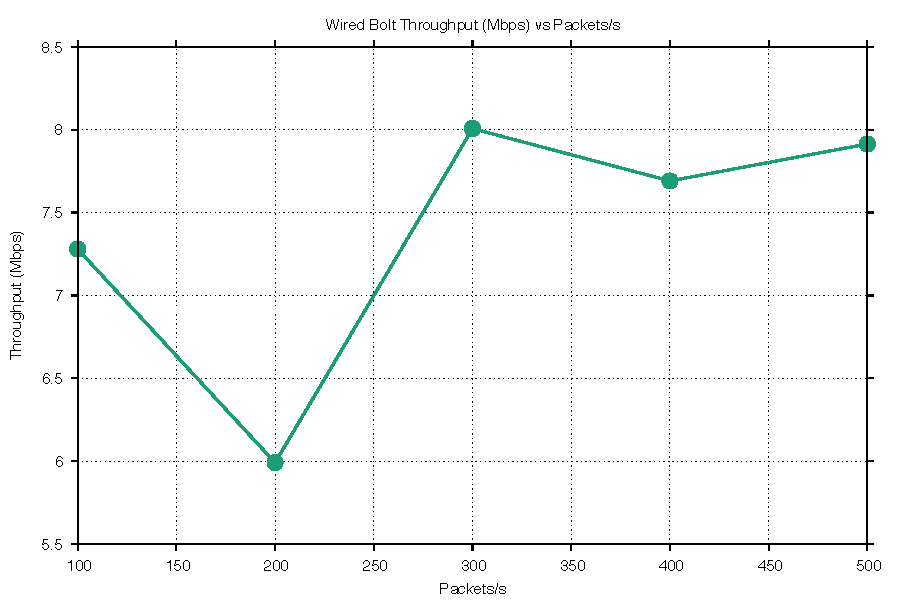
\includegraphics[width=0.78\linewidth]{project7-row7-plots/wired-throughput_mbps-pps}
\caption{Wired throughput versus packet generation rate.}
\label{fig:wired-throughput-pps}
\end{figure}

\noindent\textbf{Reason:} Throughput stays near the bottleneck limit, with small non-monotonic changes caused by timer-driven sending over the same fixed link.

\begin{figure}[t]
\centering
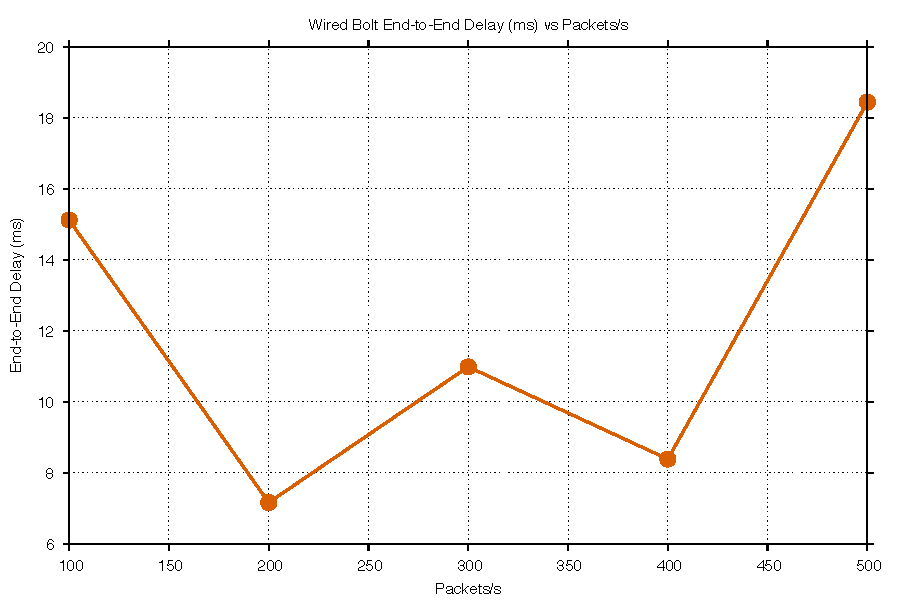
\includegraphics[width=0.78\linewidth]{project7-row7-plots/wired-avg_delay_ms-pps}
\caption{Wired average delay versus packet generation rate.}
\label{fig:wired-delay-pps}
\end{figure}

\noindent\textbf{Reason:} Delay varies with packet rate because different sending rates produce different queueing and ACK-timing interactions at the bottleneck.

\begin{figure}[t]
\centering
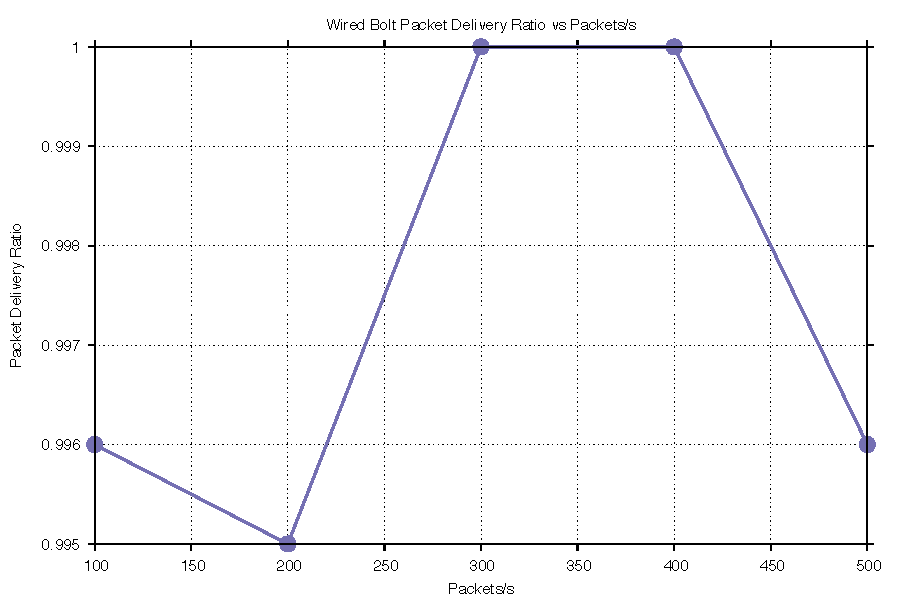
\includegraphics[width=0.78\linewidth]{project7-row7-plots/wired-pdr-pps}
\caption{Wired packet delivery ratio versus packet generation rate.}
\label{fig:wired-pdr-pps}
\end{figure}

\noindent\textbf{Reason:} PDR remains close to one because the wired path remains reliable across the tested packet rates.

\begin{figure}[t]
\centering
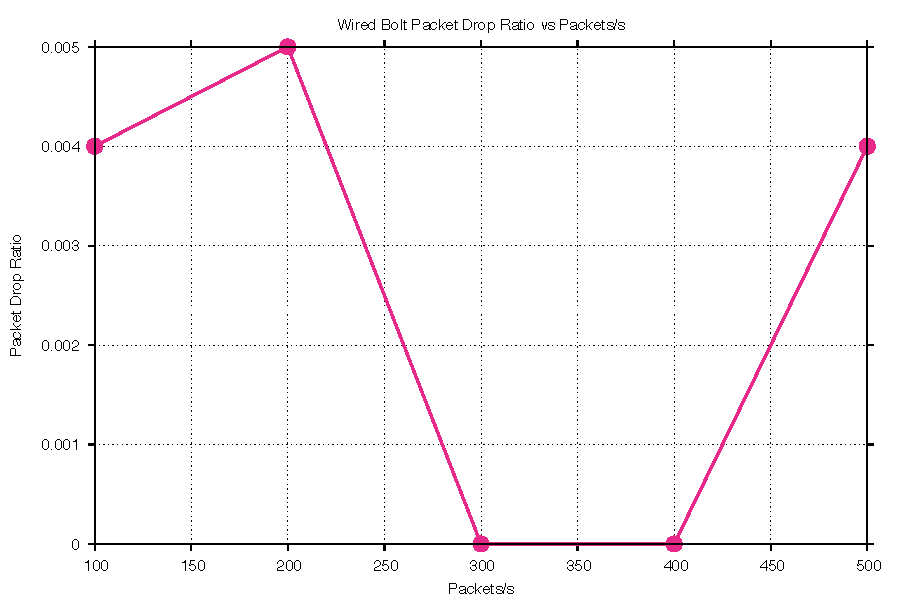
\includegraphics[width=0.78\linewidth]{project7-row7-plots/wired-drop_ratio-pps}
\caption{Wired packet drop ratio versus packet generation rate.}
\label{fig:wired-drop-pps}
\end{figure}

\noindent\textbf{Reason:} Drop ratio stays close to zero because packet-rate changes do not introduce severe loss on the wired bottleneck.

\section{Static IEEE 802.15.4 Results}

The static IEEE 802.15.4 experiment evaluates Bolt over a low-rate shared wireless medium while varying the number of nodes, the number of flows, the packet generation rate, and the coverage area. The measured metrics are throughput, average end-to-end delay, packet delivery ratio, packet drop ratio, and total network energy consumption.

\subsection{Node Sweep}

\begin{table}[t]
\centering
\small
\caption{Static IEEE 802.15.4 results for node variation.}
\label{tab:lrwpan-nodes}
\begin{tabular}{cccccc}
\hline
Nodes & Throughput (Mbps) & Delay (ms) & PDR & Drop Ratio & Energy (J) \\
\hline
20  & 0.010 & 305.760  & 0.495 & 0.505 & 24.520  \\
40  & 0.007 & 420.946  & 0.441 & 0.559 & 49.126  \\
60  & 0.005 & 659.502  & 0.348 & 0.652 & 73.889  \\
80  & 0.004 & 711.545  & 0.327 & 0.673 & 98.499  \\
100 & 0.003 & 1074.222 & 0.317 & 0.683 & 123.248 \\
\hline
\end{tabular}
\end{table}

\begin{figure}[t]
\centering
\includegraphics[width=0.78\linewidth]{project7-row7-plots/lrwpan-static-throughput_mbps-nodes}
\caption{Static IEEE 802.15.4 throughput versus number of nodes.}
\label{fig:lrwpan-throughput-nodes}
\end{figure}

\noindent\textbf{Reason:} Throughput decreases as node count grows because more nodes contend on the same low-rate shared wireless medium.

\begin{figure}[t]
\centering
\includegraphics[width=0.78\linewidth]{project7-row7-plots/lrwpan-static-avg_delay_ms-nodes}
\caption{Static IEEE 802.15.4 average delay versus number of nodes.}
\label{fig:lrwpan-delay-nodes}
\end{figure}

\noindent\textbf{Reason:} Delay increases with node count because contention, backoff, and retransmissions become more frequent.

\begin{figure}[t]
\centering
\includegraphics[width=0.78\linewidth]{project7-row7-plots/lrwpan-static-pdr-nodes}
\caption{Static IEEE 802.15.4 packet delivery ratio versus number of nodes.}
\label{fig:lrwpan-pdr-nodes}
\end{figure}

\noindent\textbf{Reason:} PDR falls as node count increases because successful packet delivery becomes harder in a denser shared channel.

\begin{figure}[t]
\centering
\includegraphics[width=0.78\linewidth]{project7-row7-plots/lrwpan-static-drop_ratio-nodes}
\caption{Static IEEE 802.15.4 packet drop ratio versus number of nodes.}
\label{fig:lrwpan-drop-nodes}
\end{figure}

\noindent\textbf{Reason:} Drop ratio rises with node count because denser contention causes more transmission failures.

\begin{figure}[t]
\centering
\includegraphics[width=0.78\linewidth]{project7-row7-plots/lrwpan-static-energy_consumption_j-nodes}
\caption{Static IEEE 802.15.4 total energy consumption versus number of nodes.}
\label{fig:lrwpan-energy-nodes}
\end{figure}

\noindent\textbf{Reason:} Total energy grows almost linearly because more wireless radios remain active for the same simulation duration.

\subsection{Flow Sweep}

\begin{table}[t]
\centering
\small
\caption{Static IEEE 802.15.4 results for flow variation.}
\label{tab:lrwpan-flows}
\begin{tabular}{cccccc}
\hline
Flows & Throughput (Mbps) & Delay (ms) & PDR & Drop Ratio & Energy (J) \\
\hline
10 & 0.004 & 281.608 & 0.420 & 0.580 & 49.232 \\
20 & 0.006 & 432.416 & 0.419 & 0.581 & 49.184 \\
30 & 0.008 & 675.306 & 0.388 & 0.612 & 49.085 \\
40 & 0.009 & 504.233 & 0.343 & 0.657 & 49.014 \\
50 & 0.009 & 840.940 & 0.345 & 0.655 & 49.018 \\
\hline
\end{tabular}
\end{table}

\begin{figure}[t]
\centering
\includegraphics[width=0.78\linewidth]{project7-row7-plots/lrwpan-static-throughput_mbps-flows}
\caption{Static IEEE 802.15.4 throughput versus number of flows.}
\label{fig:lrwpan-throughput-flows}
\end{figure}

\noindent\textbf{Reason:} Throughput rises slightly at first and then saturates because additional flows add load faster than the 802.15.4 channel can serve it.

\begin{figure}[t]
\centering
\includegraphics[width=0.78\linewidth]{project7-row7-plots/lrwpan-static-avg_delay_ms-flows}
\caption{Static IEEE 802.15.4 average delay versus number of flows.}
\label{fig:lrwpan-delay-flows}
\end{figure}

\noindent\textbf{Reason:} Delay generally increases with more flows because MAC-level contention grows on the same shared channel.

\begin{figure}[t]
\centering
\includegraphics[width=0.78\linewidth]{project7-row7-plots/lrwpan-static-pdr-flows}
\caption{Static IEEE 802.15.4 packet delivery ratio versus number of flows.}
\label{fig:lrwpan-pdr-flows}
\end{figure}

\noindent\textbf{Reason:} PDR drops as the number of flows increases because more traffic competes for the same wireless airtime.

\begin{figure}[t]
\centering
\includegraphics[width=0.78\linewidth]{project7-row7-plots/lrwpan-static-drop_ratio-flows}
\caption{Static IEEE 802.15.4 packet drop ratio versus number of flows.}
\label{fig:lrwpan-drop-flows}
\end{figure}

\noindent\textbf{Reason:} Drop ratio rises because additional flows increase queue pressure and contention losses.

\begin{figure}[t]
\centering
\includegraphics[width=0.78\linewidth]{project7-row7-plots/lrwpan-static-energy_consumption_j-flows}
\caption{Static IEEE 802.15.4 total energy consumption versus number of flows.}
\label{fig:lrwpan-energy-flows}
\end{figure}

\noindent\textbf{Reason:} Energy stays almost flat because node count and simulation time are fixed, so baseline radio-on time dominates.

\subsection{Packet-Rate Sweep}

\begin{table}[t]
\centering
\small
\caption{Static IEEE 802.15.4 results for packet-rate variation.}
\label{tab:lrwpan-pps}
\begin{tabular}{cccccc}
\hline
Packets/s & Throughput (Mbps) & Delay (ms) & PDR & Drop Ratio & Energy (J) \\
\hline
100 & 0.007 & 499.368 & 0.417 & 0.583 & 49.121 \\
200 & 0.007 & 308.200 & 0.432 & 0.568 & 49.116 \\
300 & 0.006 & 415.223 & 0.413 & 0.587 & 49.202 \\
400 & 0.007 & 322.184 & 0.388 & 0.612 & 49.097 \\
500 & 0.007 & 367.566 & 0.416 & 0.584 & 49.116 \\
\hline
\end{tabular}
\end{table}

\begin{figure}[t]
\centering
\includegraphics[width=0.78\linewidth]{project7-row7-plots/lrwpan-static-throughput_mbps-pps}
\caption{Static IEEE 802.15.4 throughput versus packet generation rate.}
\label{fig:lrwpan-throughput-pps}
\end{figure}

\noindent\textbf{Reason:} Throughput remains nearly flat because the wireless channel is already close to saturation and extra offered traffic does not translate into useful delivery.

\begin{figure}[t]
\centering
\includegraphics[width=0.78\linewidth]{project7-row7-plots/lrwpan-static-avg_delay_ms-pps}
\caption{Static IEEE 802.15.4 average delay versus packet generation rate.}
\label{fig:lrwpan-delay-pps}
\end{figure}

\noindent\textbf{Reason:} Delay stays high and irregular because higher packet rates mainly intensify contention rather than improve service rate.

\begin{figure}[t]
\centering
\includegraphics[width=0.78\linewidth]{project7-row7-plots/lrwpan-static-pdr-pps}
\caption{Static IEEE 802.15.4 packet delivery ratio versus packet generation rate.}
\label{fig:lrwpan-pdr-pps}
\end{figure}

\noindent\textbf{Reason:} PDR remains moderate and slightly unstable because packet-rate changes mostly affect contention on the shared medium.

\begin{figure}[t]
\centering
\includegraphics[width=0.78\linewidth]{project7-row7-plots/lrwpan-static-drop_ratio-pps}
\caption{Static IEEE 802.15.4 packet drop ratio versus packet generation rate.}
\label{fig:lrwpan-drop-pps}
\end{figure}

\noindent\textbf{Reason:} Drop ratio stays high because the channel remains contention-limited across the tested packet rates.

\begin{figure}[t]
\centering
\includegraphics[width=0.78\linewidth]{project7-row7-plots/lrwpan-static-energy_consumption_j-pps}
\caption{Static IEEE 802.15.4 total energy consumption versus packet generation rate.}
\label{fig:lrwpan-energy-pps}
\end{figure}

\noindent\textbf{Reason:} Energy is almost unchanged because fixed runtime and always-on radios dominate total energy consumption.

\subsection{Coverage-Area Sweep}

\begin{table}[t]
\centering
\small
\caption{Static IEEE 802.15.4 results for coverage-area variation.}
\label{tab:lrwpan-area}
\begin{tabular}{cccccc}
\hline
Area Multiplier & Throughput (Mbps) & Delay (ms) & PDR & Drop Ratio & Energy (J) \\
\hline
1$\times$ & 0.002 & 3214.368 & 0.380 & 0.620 & 49.551 \\
2$\times$ & 0.004 & 605.736  & 0.316 & 0.684 & 49.322 \\
3$\times$ & 0.007 & 437.332  & 0.443 & 0.557 & 49.160 \\
4$\times$ & 0.008 & 397.817  & 0.479 & 0.521 & 49.045 \\
5$\times$ & 0.009 & 339.160  & 0.463 & 0.537 & 49.037 \\
\hline
\end{tabular}
\end{table}

\begin{figure}[t]
\centering
\includegraphics[width=0.78\linewidth]{project7-row7-plots/lrwpan-static-throughput_mbps-area}
\caption{Static IEEE 802.15.4 throughput versus coverage area.}
\label{fig:lrwpan-throughput-area}
\end{figure}

\noindent\textbf{Reason:} Throughput improves with larger area because spatial separation reduces interference while keeping the network sufficiently connected.

\begin{figure}[t]
\centering
\includegraphics[width=0.78\linewidth]{project7-row7-plots/lrwpan-static-avg_delay_ms-area}
\caption{Static IEEE 802.15.4 average delay versus coverage area.}
\label{fig:lrwpan-delay-area}
\end{figure}

\noindent\textbf{Reason:} Delay drops sharply as area increases because fewer collisions and retries reduce waiting time.

\begin{figure}[t]
\centering
\includegraphics[width=0.78\linewidth]{project7-row7-plots/lrwpan-static-pdr-area}
\caption{Static IEEE 802.15.4 packet delivery ratio versus coverage area.}
\label{fig:lrwpan-pdr-area}
\end{figure}

\noindent\textbf{Reason:} PDR improves overall with larger area because reduced medium contention increases successful delivery.

\begin{figure}[t]
\centering
\includegraphics[width=0.78\linewidth]{project7-row7-plots/lrwpan-static-drop_ratio-area}
\caption{Static IEEE 802.15.4 packet drop ratio versus coverage area.}
\label{fig:lrwpan-drop-area}
\end{figure}

\noindent\textbf{Reason:} Drop ratio decreases as area grows because wider spacing lowers interference on the shared channel.

\begin{figure}[t]
\centering
\includegraphics[width=0.78\linewidth]{project7-row7-plots/lrwpan-static-energy_consumption_j-area}
\caption{Static IEEE 802.15.4 total energy consumption versus coverage area.}
\label{fig:lrwpan-energy-area}
\end{figure}

\noindent\textbf{Reason:} Energy decreases slightly with larger area because fewer retransmissions reduce additional radio activity.
